% Figure 5.12: Laravel-Julia Integration Architecture
% Compile with: pdflatex fig_5_12_integration_architecture.tex

\documentclass[border=10pt]{standalone}
\usepackage{tikz}
\usetikzlibrary{shapes.geometric, arrows.meta, positioning}
\usepackage{xcolor}

% Professional academic color palette
\definecolor{primaryblue}{RGB}{70, 130, 180}   % Steel blue
\definecolor{secondarygray}{RGB}{119, 136, 153} % Light slate gray
\definecolor{accentteal}{RGB}{119, 176, 166}   % Muted teal
\definecolor{lightfill}{RGB}{245, 245, 245}    % Very light gray
\definecolor{databg}{RGB}{220, 220, 220}
\definecolor{textdark}{RGB}{33, 33, 33}

\begin{document}
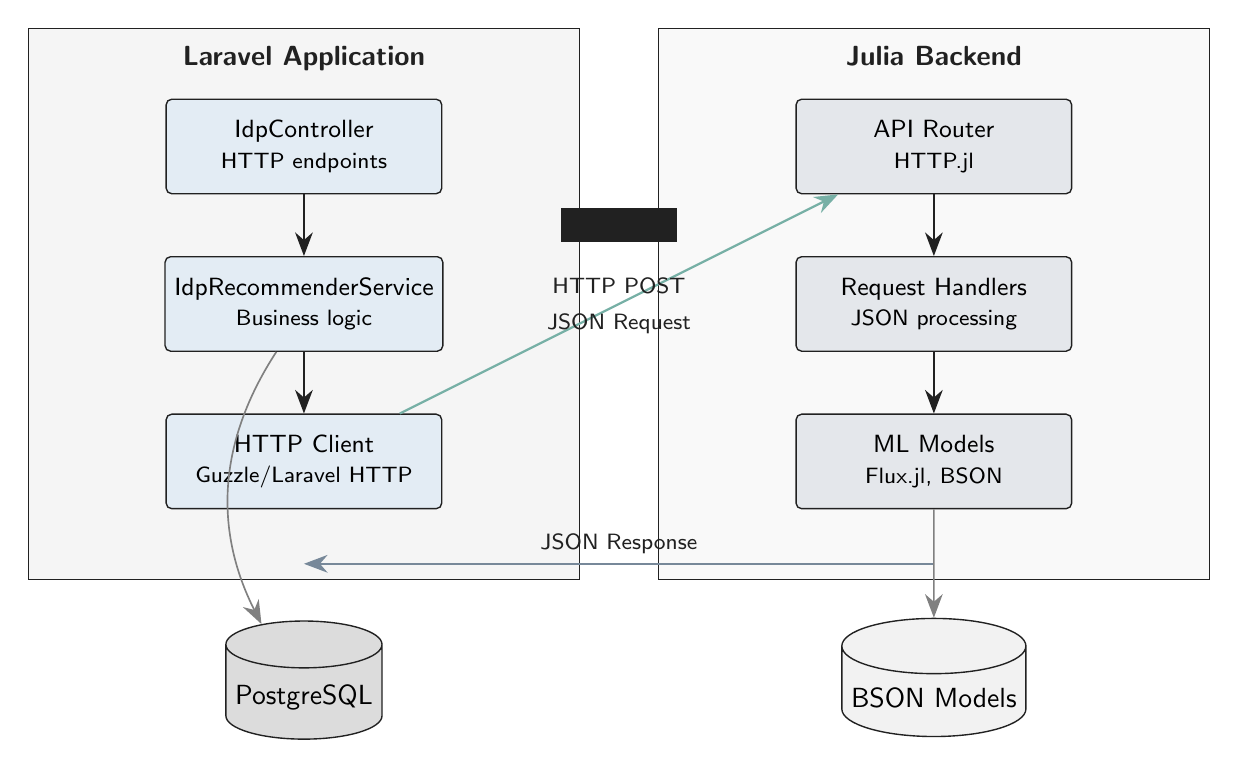
\begin{tikzpicture}[
    node distance=1.5cm,
    component/.style={rectangle, draw=textdark, rounded corners=2pt, minimum width=3.5cm, minimum height=1.2cm, align=center, font=\small\sffamily, line width=0.5pt},
    arrow/.style={-{Stealth[length=3mm]}, semithick, color=textdark},
]

% Laravel side
\node[rectangle, draw=textdark, fill=lightfill, minimum width=7cm, minimum height=7cm, line width=0.5pt] (laravelbox) at (-4, 3.5) {};
\node[font=\bfseries\sffamily, anchor=north, color=textdark] at (-4, 6.9) {Laravel Application};

\node[component, fill=primaryblue!15] (controller) at (-4, 5.5) {IdpController\\{\footnotesize\sffamily HTTP endpoints}};
\node[component, fill=primaryblue!15] (service) at (-4, 3.5) {IdpRecommenderService\\{\footnotesize\sffamily Business logic}};
\node[component, fill=primaryblue!15] (http) at (-4, 1.5) {HTTP Client\\{\footnotesize\sffamily Guzzle/Laravel HTTP}};

\draw[arrow] (controller) -- (service);
\draw[arrow] (service) -- (http);

% Julia side
\node[rectangle, draw=textdark, fill=gray!5, minimum width=7cm, minimum height=7cm, line width=0.5pt] (juliabox) at (4, 3.5) {};
\node[font=\bfseries\sffamily, anchor=north, color=textdark] at (4, 6.9) {Julia Backend};

\node[component, fill=secondarygray!20] (router) at (4, 5.5) {API Router\\{\footnotesize\sffamily HTTP.jl}};
\node[component, fill=secondarygray!20] (handlers) at (4, 3.5) {Request Handlers\\{\footnotesize\sffamily JSON processing}};
\node[component, fill=secondarygray!20] (models) at (4, 1.5) {ML Models\\{\footnotesize\sffamily Flux.jl, BSON}};

\draw[arrow] (router) -- (handlers);
\draw[arrow] (handlers) -- (models);

% Connection
\draw[arrow, accentteal, thick] (http) -- node[above, font=\footnotesize\sffamily, color=textdark] {HTTP POST} node[below, font=\footnotesize\sffamily, color=textdark] {JSON Request} (router);

% Response arrow
\draw[arrow, secondarygray, thick] (4, 0.2) -- node[above, font=\footnotesize\sffamily, color=textdark] {JSON Response} (-4, 0.2);

% Database
\node[cylinder, draw=textdark, fill=databg, shape border rotate=90, aspect=0.3, minimum height=1.5cm, font=\sffamily, line width=0.5pt] (db) at (-4, -1.5) {PostgreSQL};
\draw[arrow, gray] (service) to[bend right=30] (db);

% Model files
\node[cylinder, draw=textdark, fill=gray!10, shape border rotate=90, aspect=0.3, minimum height=1.5cm, font=\sffamily, line width=0.5pt] (bson) at (4, -1.5) {BSON Models};
\draw[arrow, gray] (models) -- (bson);

% Port annotation
\node[font=\footnotesize\sffamily, fill=white, color=textdark] at (0, 4.5) {Port 8080};

\end{tikzpicture}
\end{document}
